\documentclass[10pt,a4paper,titlepage]{article}
\usepackage[utf8]{inputenc}
\usepackage{amsmath}
\usepackage{amsfonts}
\usepackage{amssymb}
\usepackage[ngerman]{babel}
\usepackage[pdftex]{graphicx}
\usepackage[vmargin=3cm, hmargin=2cm]{geometry}
\usepackage{tabularx}
\usepackage{fancyvrb}
\usepackage{pdflscape}

\setlength{\parindent}{0pt}
\setlength{\parskip}{2pt}

\title{Entwurfsdokument}
\author{Simon Bischof \and Jan Haag \and Adrian Herrmann \and Lin Jin \and Tobias Schlumberger \and Matthias Schnetz}

\makeindex

\begin{document}

\thispagestyle{empty}
\vspace*{4cm}
\begin{center}
\begin {huge}
Entwurfsdokument\\
\end{huge}
Simon Bischof, Jan Haag, Adrian Herrmann, Lin Jin, Tobias Schlumberger, Matthias Schnetz\\
\vspace{3cm}
\begin{huge}
Praxis der Softwareentwicklung \\
Projekt 3:\\
Automatisches Pr\"{u}fen der Korrektheit von Programmen\\
Gruppe 1\\
\vspace{2cm}
\includegraphics[height=2cm]{images/Logo.pdf}\\[0.5cm]
\end{huge}
\begin{huge}
WS 2011/2012
\end{huge}
\end{center}
\newpage
\tableofcontents
\newpage

\section{Klassendiagramme}

\subsection{"Ubersicht}

Das folgende Klassendiagramm zeigt die Interaktionen zwischen den Komponenten des Systems. \\
\includegraphics[scale=0.85]{images/ClassOverview.pdf} \\
Die gesamte Architektur basiert auf dem Entwurfsmuster Model-View-Controller. Dies erm"oglicht uns einen flexiblen Programmentwurf, der eine sp"atere "Anderung oder Erweiterung erleichtert und eine Wiederverwendbarkeit der einzelnen Komponenten erm"oglicht.
\begin{itemize}
\item Das \textbf{Modell} enth"alt die darzustellenden Daten, z.B die Zust"ande der Variablen w"ahrend der Programmausf"uhrung und die vom Benutzer gesetzten Breakpoints. Aber auch die Komponenten AST und Miscellaneous sind Bestandteile des Modells. Diese Speichern jeweils den Syntaxbaum des Benutzerprogramms und wichtige Daten der Benutzeroberfl"ache. 
\item Die \textbf{Sicht} stellt die Daten, die sie vom Modell bekommt, auf der Benutzeroberfl"ache dar und nimmt Benutzerinteraktionen entgegen. Dabei wird sie unterteilt in verschiedenen Views, wie zum Beispiel die VariableView und BreakpointView. 
\item Um die Zusammenarbeit der ersten zwei Komponenten k"ummert sich die \textbf{Steuerung}. Da wir mehrere Views haben, gibt es dementsprechend auch mehrere Controller. Diese steuern alle Komponenten des Systems und geben Daten weiter. Wichtige Aufgaben der Steuerung sind beispielsweise das Aufrufen des Parsers und des Interpreters. \\
\end{itemize}

\subsection{Feinstruktur der Komponenten}

\subsubsection{AST}

%\includegraphics[scale=0.55]{images/AST.pdf} \\
F"ur die Struktur des AST verwenden wir das Composite-Muster. Damit wird die Teil-Ganzes-Hierachie der While-Grammatik repr"asentiert, indem Objekte zu Baumstrukturen zusammengef"ugt werden. Au"serdem erm"oglicht uns das Muster, Objekte und Kompositionen einheitlich zu behandeln. Um die Methoden des Interpreters, des Type-Checkers und des Beweisers zu kapseln, verwenden wir hier auch das Visitor-Muster. Somit k"onnen diese Methoden leicht f"ur alle konkreten Klassen implementiert werden und auch einfacher modifiziert werden. 
\begin{itemize}
\item \texttt{ASTRoot} \\
Die Klasse ASTRoot bildet die Wurzel des Baumes. Sie wird direkt vom Parser erzeugt und wird zum Verifizieren an den Beweiser "ubergeben. 
\begin{itemize}
\item Attribut: \\
\texttt{position} \\
eine bestimmte Position im Quelltext
\item Methoden: \\
\texttt{getPosition()} \\
gibt \texttt{position} zur"uck \\
\texttt{acceptVisitor(visitor: ASTVisitor)} \\
nimmt einen konkreten Visitor entgegen
\end{itemize}
\item \texttt{Program} \\
Die Klasse \texttt{Program} ist eine Ansammlung von Funktionen. 
\begin{itemize}
\item Attribute: \\
\texttt{functions} \\
\texttt{Program} besteht aus einer oder mehreren Funktionen\\
\texttt{mainFunction} \\
\texttt{Program} muss aus genau einer Main-Funktion besthen \\
\texttt{axioms} \\
\texttt{Program} kann auch Axiome enthalten
\item Methoden: \\
\texttt{getFunctions()} \\
gibt die Menge der Funktionen zur"uck \\
\texttt{getMainFunction()} \\
gibt \texttt{mainFunction} zur"uck \\
\texttt{getGlobalAxioms()} \\
gibt die Menge der globalen Axiomen zur"uck
\end{itemize}
\item \texttt{Function} \\
Die Klasse \texttt{Function} stellt eine Funktion im Programmcode dar. 
\begin{itemize}
\item Attribute: \\
\texttt{name} \\
der Name der Funktion \\
\texttt{parameters} \\
beliebig viele Parameter \\
\texttt{returnType} \\
R"uckgabetyp der Funktion \\
\texttt{functionBody} \\
eine Funktion besteht einem \texttt{StatementBlock} \\
\item Methoden: \\
\texttt{getFunctionBlock()} \\
gibt den K"orper der Funktion als \texttt{StatementBlock} zur"uck \\
\texttt{getParameters()} \\
gibt die Menge der Parameter zur"uck \\
\texttt{getName()} \\
gibt \texttt{name} zur"uck \\
\texttt{getReturnType()} \\
gibt \texttt{returnType} zur"uck 
\end{itemize}
\item \texttt{FunctionParameter}
\begin{itemize}
\item Attribute: \\
\texttt{identifier} \\
der Name des Parameters 
\texttt{type} \\
\texttt{Parameter} muss einen Typ haben
\item Methoden: \\
\texttt{getName()} \\
gibt \texttt{identifier} zur"uck \\
\texttt{getType} \\
gibt \texttt{type} zur"uck
\end{itemize}
\item \texttt{StatementBlock} \\
Die Klasse \texttt{StatementBlock} kapselt eine logische zusammengehörende Liste von \texttt{Statements}.
\begin{itemize}
\item Attribute: \\
\texttt{statements} \\
eine geordnete Liste von \texttt{Statements} \\
\item Methoden: \\
\texttt{getNextStatement()} \\
gibt das nächste Statement zurück, oder NULL, falls das Ende des Blocks erreicht wurde.
\end{itemize}
\item \texttt{Statement} \\
Die Klasse \texttt{Statement} steht f"ur eine Anweisung im Programmcode. 
\item \texttt{Conditional} \\
Die Klasse \texttt{Conditional} ist eine Unterklasse von \texttt{Statement} und steht f"ur eine bedingte Anweisung. 
\begin{itemize}
\item Attribute: \\
\texttt{trueStatements} \\
es gibt einen \texttt{StatementBlock}, der bei Erf"ullung der Bedingung ausgef"uhrt wird \\
\texttt{falseStatements} \\
es gibt einen \texttt{StatementBlock}, der bei Nichterf"ullung der Bedingung ausgef"uhrt wird \\
\texttt{condition} \\
Bedingung, die "uberpr"uft wird
\item Methoden: \\
\texttt{getCondition()} \\
gibt \texttt{condition} zur"uck \\
\texttt{getTrueConditionBody()} \\
gibt \texttt{trueStatements} zur"uck \\
\texttt{getFalseConditionBody()} \\
gibt \texttt{falseStatements} zur"uck
\end{itemize}
\item \texttt{Loop} \\
Die Klasse \texttt{Loop} ist eine Unterklasse von \texttt{Statement} und steht f"ur eine while-Anweisung. 
\begin{itemize}
\item Attribute: \\
\texttt{body} \\
Schleifenk"orper, der bedingt ausgef"uhrt wird, solange \texttt{condition} wahr ist \\
\texttt{condition} \\
Bedingung, die "uberpr"uft wird \\
\texttt{invariant} \\
f"ur die Schleife ist es m"oglich, eine oder mehrere Schleifeninvarianten anzugeben 
\end{itemize}
\item \texttt{Specification}
\begin{itemize}
\item Attribut: \\
\texttt{expression} \\
Ausdruck, der "uberpr"uft wird
\end{itemize}
\item \texttt{ReturnStatement} \\
Die Klasse \texttt{ReturnStatement} stellt eine return-Anweisung dar. 
\begin{itemize}
\item Attribut: \\
\texttt{returnValue} \\
Ausdruck, dessen Wert zur"uckgegeben wird 
\item Methode: \\
\texttt{getReturnValue} \\
gibt \texttt{returnValue} zur"uck
\end{itemize}
\item \texttt{Assignment} \\
Die Klasse \texttt{Assignment} steht f"ur eine Zuweisung von Variablen.
\begin{itemize}
\item Attribute: \\
\texttt{value} \\
der Wert der zugewiesen werden soll \\
\texttt{identifier} \\
Variable, der \texttt{value} zugewiesen wird
\item Methoden: \\
\texttt{getValue()} \\
gibt \texttt{value} zur"uck \\
\texttt{getVariable()} \\
gibt \texttt{identifier} zur"uck
\end{itemize}
\item \texttt{VariableDeclaration}
\begin{itemize}
\item Attribute: \\
\texttt{name} \\
Name der Variable \\
\texttt{value} \\
bei der Deklaration muss genau ein Wert eines Ausdrucks zugewiesen werden \\
\texttt{type} \\
Typ der Variable 
\item Methoden: \\
\texttt{getName()} \\
gibt \texttt{name} zur"uck \\
\texttt{getValue()} \\
gibt \texttt{value} zur"uck \\
\texttt{getType()} \\
gibt \texttt{type} zur"uck
\end{itemize}
\item \texttt{Expression} \\
Die Klasse \texttt{Expression} steht f"ur einen Ausdruck im Programmcode. 
\item \texttt{LogicalExpression} \\
Die Klasse \texttt{LogicalExpression} steht f"ur einen un"aren oder bin"aren Ausdruck, der einen Booleanwert zur"uckgibt.
\begin{itemize}
\item Attribute: \\
\texttt{subExpression} \\
ein logischer Ausdruck kann als Operanden wieder Ausdr"ucken haben \\
\texttt{quantifier} \\
ein logischer Ausdruck kann einen forall- oder exists-Quantor haben \\
\texttt{logicalOperator} \\
ein logischer Ausdruck muss einen Operator aus \texttt{\{!, |, \&, >, >=, <, <=, !=, ==\}} besitzen 
\end{itemize}
\item \texttt{QuantifiedExpression} \\
Die Klasse \texttt{QuantifiedExpression} steht f"ur einen Ausdruck, der einen Quantifier enth"alt.
\item \texttt{ArithmeticExpression} \\
Die Klasse \texttt{ArithmeticExpression} steht f"ur einen un"aren oder bin"aren Ausdruck, der einen Zahlenwert zur"uckgibt.
\begin{itemize}
\item Attribute: \\
\texttt{subExpression} \\
ein arithmetischer Ausdruck kann als Operanden wieder Ausdr"ucken haben \\
\texttt{arithmeticOperator} \\
ein arithmetischer Ausdruck muss einen Operator aus \texttt{\{+, -, *, /, \%\}} besitzen 
\end{itemize}
\item \texttt{FunctionCall} \\
Die Klasse \texttt{FunctionCall} modelliert einen Methodenaufruf. 
\begin{itemize}
\item Attribute: \\
\texttt{function} \\
Funktion, die aufgerufen wird \\
\texttt{parameters} \\
Menge von Ausdr"ucken, die als Parameter der Methode "ubergeben werden
\end{itemize}
\item \texttt{VariableRead} \\
Die Klasse \texttt{VariableRead} stellt einen Zugriff auf eine Variable dar.
\begin{itemize}
\item Attribut: \\
\texttt{identifier} \\
Variable, die gelesen wird
\item Methode: \\
\texttt{getVariable()} \\
gibt \texttt{identifier} zur"uck
\end{itemize}
\item \texttt{Identifier} \\
Die Klasse \texttt{Identifier} steht f"ur eine Variable. 
\begin{itemize}
\item Attribut: \\
\texttt{name} \\
Name der Variable 
\item Methode: \\
\texttt{getName()} \\
gibt \texttt{name} zur"uck  
\end{itemize}
\item \texttt{Position} \\
Die Klasse \texttt{Position} stellt eine Position im Programmcode dar. 
\begin{itemize}
\item Attribute: \\
\texttt{line} \\
Zeile im Code \\
\texttt{column} \\
Spalte im Code \\
\end{itemize}
\end{itemize}

\subsubsection{Parser}

%\includegraphics[scale=0.3]{images/Parser.pdf} \\
Der Parser liefert die AST-Struktur f"ur den Interpreter und Beweiser. Einige Klassen dieser Komponente werden vom Parsergenerator ANTLR erstellt. 
\begin{itemize}
\item \texttt{ParserInterface} \\
Die Klasse \texttt{ParserInterface} dient als Schnittstelle zwischen der Komponente Parser und dem restlichen System. Sie wird vom Main-Controller der GUI initialisiert. 
\begin{itemize}
\item Attribute: \\
\texttt{parser} \\
Parser f"ur den Programmcode \\
\texttt{lexer} \\
Lexer f"ur den Programmcode 
\item Methode: \\
\texttt{parse(text: String)} \\
Initialisiert Parser und Lexer, "uber gibt ihnen den Quelltext
\end{itemize}
\item \texttt{Parser} \\
Die Klasse \texttt{Parser} ist f"ur die Erzeugung des AST zust"andig. Es wird eine \texttt{ParseException} geworfen, falls kein AST erzeugt werden kann. 
\item \texttt{Lexer} \\
Die Klasse \texttt{Lexer} zerlegt den Quelltext in Tokens. 
\begin{itemize}
\item Attribut: \\
\texttt{source} \\
der vom Benutzer eingegebene Quelltext 
\item Methoden: \\
\texttt{Lexer(source:String)} \\
Konstruktor der Klasse. Bei der Instanzierung wird der Quelltext "ubergeben. \\
\texttt{getSource()} \\
gibt den Quelltext zur"uck \\
\end{itemize}
\end{itemize}

\subsubsection{Interpreter}

%\includegraphics[scale=0.21]{images/Interpreter.pdf} \\
F"ur die Integration des Interpreters verwenden wir das Visitor-Muster. Es kapselt die Operationen, die auf Elementen des AST ausgef"uhrt werden. Das Muster erm"oglicht uns, Operationen zu ver"andern oder neue Funktionen hinzuf"ugen, ohne die Elementklassen zu modifizieren. Im obigen Klassendiagramm ist auch ein Teil des Modells dargestellt. Diese speichern wichtige Daten bez"uglich der Programmausf"uhrung. 
\begin{itemize}
\item \texttt{ASTVisitor} \\
Das Interface \texttt{ASTVisitor} deklariert f"ur jede Klasse konkreter Elemente eine Besuchsfunktion.
\item \texttt{TypeChecker} \\
Die Klasse \texttt{TypeChecker} ist ein konkreter Besucher und implementiert die Aufgabe, die Korrektheit der Typen zu "uberpr"ufen. Wenn ein Typfehler gefunden wird, so wird man durch eine \texttt{IllegalTypeException} benachrichtigt. 
\begin{itemize}
\item Methode: \\
\texttt{checkTypes()} \\
startet den Vorgang des Type-Checks 
\end{itemize}
\item \texttt{Interpreter} \\
Die Klasse \texttt{Interpreter} ist ein konkreter Besucher und implementiert die Aufgaben des Interpretierens. Ist die Bedingung einer Assert-Anweisung nicht erf"ullt, so wird eine \texttt{AssertFailureException} geworfen.
\begin{itemize}
\item Methode: \\
\texttt{step(state:State)} \\
schrittweise Ausf"uhrung des Programms. Dabei wird der Funktion der aktuellen Zustand \texttt{state} "ubergeben und diese gibt wieder eine Instanz der Klasse \texttt{State} zur"uck. 
\end{itemize}
\item \texttt{SMTLibTranslator} \\
Die Klasse \texttt{SMTLibTranslator} ist ein konkreter Besucher und implementiert die Aufgabe, den AST in die von Z3 ben"otigte Sprache zu "ubersetzen.
\begin{itemize}
\item Methode: \\
\texttt{getWPTree(ast: ASTRoot)} \\
"ubersetzt den AST in ein \texttt{WPProgram}
\end{itemize}
\item \texttt{State} \\
Die Klasse \texttt{State} speichert den aktuellen Zustand der Programmausf"uhrung, wie z.B. Werte von Variablen.
\begin{itemize}
\item Attribute: \\
\texttt{statement} \\
jedem Zustand ist ein Statement zugeordnet \\
\texttt{currentScope} \\
die erste Scope-Instanz, die instanziert wurde
\item Methoden: \\
\texttt{createScope()} \\
erzeugt f"ur eine Variable die entsprechende \texttt{Scope}-Instanz \\
\texttt{destroyScope()} \\
zerst"ort eine \texttt{Scope}-Instanz \\
\texttt{setVar(name: String,value:String)}  \\
setzt eine Variable und ihren Wert \\
\texttt{createVar(name: String,value:String,type: TypeOfValue)} \\
erstellt eine Variable mit einem Typ und Wert
\end{itemize}
\item \texttt{Scope} \\
Die Klasse \texttt{Scope} bildet eine Hierachie der Sichtbarkeit von Variablen des Programms. Je weiter unten sich eine \texttt{Scope}-Instanz befindet, desto lokaler ist die damit verbundenen Variable. In der obersten Ebene befinden sich also die globalen Variablen. Bei einem Variablenzugriff wird zun"achst die unterste Ebene "uberpr"uft, ob diese die gesuchte Variable enth"alt. Wenn dies nicht der Fall ist, so sucht man in der n"achst h"oheren Ebene weiter. Wenn man bereits die oberste Ebene erfolglos durchsucht hat, ist die Variable nicht vorhanden und eine Exception wird geworfen. 
\begin{itemize}
\item Attribut: \\
\texttt{upScope} \\
nur die erste Scope-Instanz wird von \texttt{State}, alle weiteren werden von der Klasse selbst verwaltet \\
\item Methode: \\
\texttt{getParent()} \\
gibt die "`Eltern"'-Instanz \texttt{upScope} zur"uck \\
\texttt{getNextStatement()} \\
gibt das n"achste \texttt{Statement} zur"uck \\
\texttt{addVars(<Identifier, Value>*)} \\
f"ugt im untersten Scope alle Variablen hinzu, in den dar"uberliegenden Scopes nur noch die nicht vorhandenen \\
\end{itemize}
\item \texttt{Value} \\
Die Klasse \texttt{Value} speichert den Wert einer zugeh"origen Variable. 
\begin{itemize}
\item Attribute: \\
\texttt{type} \\
Typ des Wertes \\
\texttt{identifier} \\
Name der Variable 
\item Methode: \\
\texttt{getType()} \\
gibt \texttt{type} zur"uck 
\end{itemize}
\item \texttt{Breakpoint}
\begin{itemize}
\item Attribut: \\
\texttt{active} \\
boolsche Variable, die anzeigt, ob der Breakpoint aktiviert ist \\
\item Methoden: \\
\texttt{setActive(active:boolean)} \\
aktiviert oder deaktiviert den Breakpoint \\
\texttt{isActive()} \\
gibt \texttt{active} zur"uck
\end{itemize}
\item \texttt{StatementBreakpoint} \\
Die Klasse \texttt{StatementBreakpoint} ist eine Unterklasse von \texttt{Breakpoint} und stellt einen Breakpoint dar, der an einer bestimmten Stelle im Quellcode steht. 
\begin{itemize}
\item Attribut: \\
\texttt{statement} \\
Anweisung, an der der Breakpoint gebunden ist
\item Methode: \\
\texttt{getStatement()} \\
gibt \texttt{statement} zur"uck
\end{itemize}
\item \texttt{GlobalBreakpoint} \\
Die Klasse \texttt{GlobalBreakpoint} ist eine Unterklasse von \texttt{Breakpoint} und stellt einen globalen Breakpoint dar, der an einem Ausdruck gebunden ist und nicht an einer bestimmten Stelle im Programmcode. 
\begin{itemize}
\item Attribut: \\
\texttt{expression} \\
logischer Ausdruck, an dem der globale Breakpoint gebunden ist
\item Methode: \\
\texttt{getExpression()} \\
gibt \texttt{expression} zur"uck 
\end{itemize}
\item \texttt{ProgramExecution} \\
Die Klasse \texttt{ProgramExecution} modelliert die Programmausf"uhrung.
\begin{itemize}
\item Attribute: \\
\texttt{breakpoints} \\
\texttt{ProgramExecution} ist f"ur die "Uberpr"ufung der Breakpoints zust"andig \\
\texttt{position} \\
\texttt{ProgramExecution} hat zu einem Zeitpunkt eine bestimmte Position im Quellcode 
\item Methoden: \\
\texttt{ProgramExecution(interpreter: Interpreter)} \\
Konstruktor, der Interpreter wird dabei "ubergeben \\
\texttt{checkBreakpoint()} \\
"uberpr"uft, ob ein Breakpoint getroffen wurde \\
\texttt{setBreakpoint(active: Boolean, pos: Position)} \\
setzt einen aktiven oder inaktiven Breakpoint an die Position pos \\
\texttt{getVariables()} \\
gibt alle Variablen und ihren Werten zur"uck
\end{itemize}
\item \texttt{MessageSystem} \\
Die Klasse \texttt{MessageSystem} leitet R"uckmeldungen (z.B. Fehlermeldungen) an die GUI weiter. 
\begin{itemize}
\item Attribut: \\
\texttt{consoles} \\
Das Message-System hat bestimmte Konsolen gespeichert, denen es Nachrichten "ubermitteln soll 
\item Methoden: \\
\texttt{addConsole(console: Console)} \\
f"ugt console zur Liste der zu benachrichtigenden Konsolen hinzu \\
\texttt{removeConsole(console: Console)} \\
entfert console aus der Liste \\
\texttt{sendUpdate()} \\
benachrichtigt Konsolen "uber Ver"anderungen \\
\end{itemize}
\end{itemize}

\subsubsection{Beweiser}

%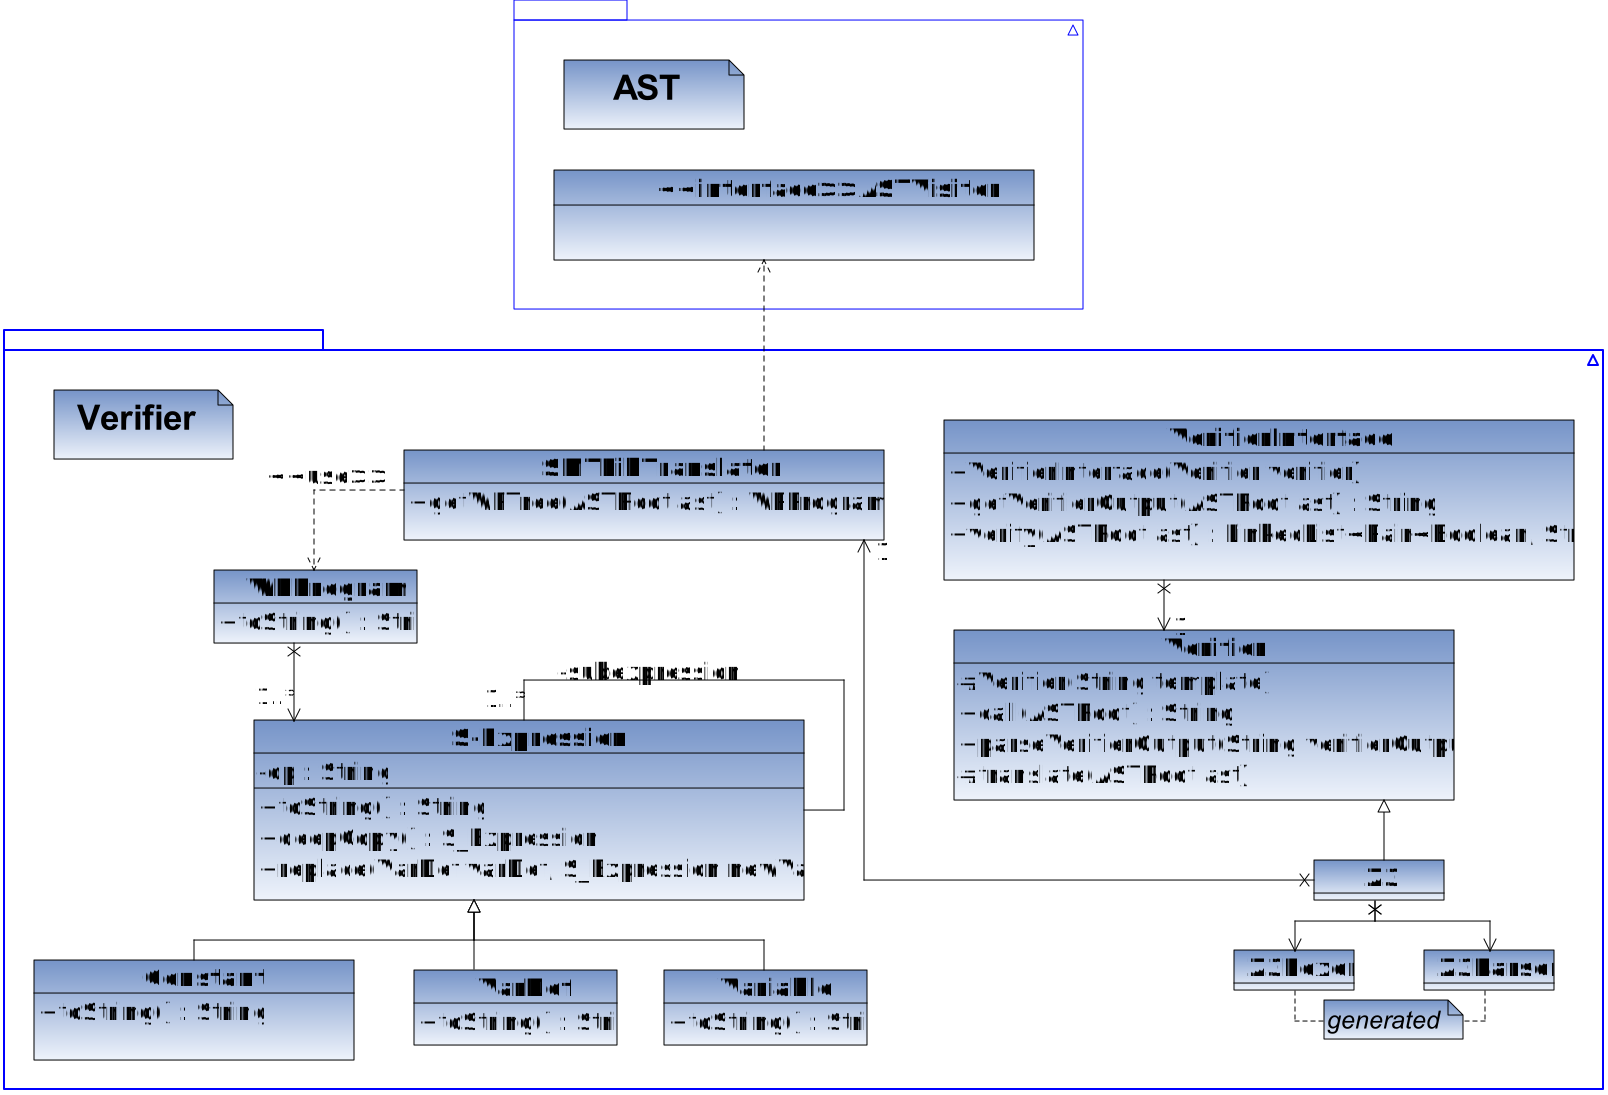
\includegraphics[scale=0.3]{images/Verifier.pdf} \\
Die Komponente Verifier "ubersetzt den AST in eine Struktur, die die Weakest-Precondition generiert. ANTLR hilft uns auch hier, die ben"otigten Lexer- und Parserklassen zu erzeugen. 
\begin{itemize}
\item \texttt{VerifierInterface} \\
Die Klasse \texttt{VerifierInterface} stellt die Schnittstelle zwischen der Komponente Verifier und dem restlichen System dar. Sie wird vom Main-Controller initialisiert und startet die "Ubersetzung des SMTLibTranslators. 
\begin{itemize}
\item Attribute: \\
\texttt{smtlibTranslator} \\
"Ubersetzer, der den AST "ubersetzen soll \\
\texttt{program} \\
Programm in der wp-Struktur \\
\texttt{z3lexer} \\
Lexer f"ur Z3-Ergebnis \\
\texttt{z3parser} \\
Parser f"ur Z3-Ergebnis \\
\item Methoden: \\
\texttt{notifyConsole()} \\
benachrichtigt Konsolen "uber Beweisergebnisse \\
\texttt{verify(ast: ASTRoot)} \\
startet die "Ubersetzung
\end{itemize}
\item \texttt{S-Expression} \\
Die Klasse \texttt{S-Expression} stellt einen beliebigen Ausdruck dar. 
\begin{itemize}
\item Attribute: \\
\texttt{op} \\
Operator des Ausdrucks \\
\texttt{subexpression} \\
Operanden sind wieder S-Expressions 
\item Methode: \\
\texttt{toString()} \\
gibt eine Strinrepr"asentation zur"uck als R"uck"ubersetzung 
\end{itemize}
\item \texttt{Constant} \\
Die Klasse \texttt{Constant} ist eine Unterklasse von \texttt{S-Expressions} und bildet das Blatt des Composite-Musters. 
\begin{itemize}
\item Attribut: \\
\texttt{stringRepr"asentation} \\
die Konstante als String \\
\end{itemize}
\end{itemize}

\subsubsection{Misc}

%\includegraphics[scale=0.27]{images/Misc.pdf}\\
In dieser Komponente werden Daten, die der Benutzeroberfl"ache betreffen, gespeichert. 
\begin{itemize}
\item \texttt{FileManagement} \\
Die Klasse \texttt{FileManagement} k"ummert sich um das Speichern von Benutzerdateien. 
\begin{itemize}
\item Methoden: \\
\texttt{loadFile(dir: String)} \\
l"adt eine Datei \\
\texttt{saveFile(text: String, dir: String)} \\
speichert Programm in eine Datei 
\end{itemize}
\item \texttt{About} \\
Die Klasse \texttt{About} speichert n"utzliche Informationen zu unserem Produkt. 
\begin{itemize}
\item Attribut: \\
\texttt{text} \\
wichtiger Text \\
\texttt{singleton} \\
Singleton-Muster, da der Text nicht mehrmals erzeugt werden muss 
\item Methoden: \\
\texttt{getInstance()} \\
gibt \texttt{singleton} zur"uck \\
\texttt{getText()} \\
gibt \texttt{text} zur"uck
\end{itemize}
\item \texttt{Settings} \\
Die Klasse \texttt{Settings} speichert Einstellungen f"ur den Beweiser. 
\begin{itemize}
\item Attribute: \\
\texttt{timeout} \\
Zeitlimit f"ur einen Beweisvorgang \\
\texttt{memorylimit} \\
Speicherlimit f"ur einen Beweisvorgang 
\end{itemize}
\end{itemize}

\subsubsection{Benutzeroberfl"ache}

%\includegraphics[scale=0.27]{images/GUI.pdf} \\
Die Benutzeroberfl"ache bietet dem Benutzer eine leicht zu bedienende Schnittstelle und nimmt dessen Eingaben entgegen. Um die verschiedenen Sichten zu steuern, gibt es f"ur jede Sicht einen eigenen Controller. "Uber diese Controllers geschehen alle Interaktionen mit anderen Komponenten, z.B. reichen sie Benutzereingaben weiter, damit diese verarbeitet werden k"onnen. Die Controllers stellen der Views auch die von ihr ben"otigten Informationen zur Verf"ugung. 
\begin{itemize}
\item \texttt{MainController} \\
Die Klasse \texttt{MainController} ist zust"andig f"ur die Initialisierung des Parsers, des TypeCheckers, des Beweisers und des Message-Systems zust"andig. Sie erzeugt au"serdem auch noch die Main-Frame.
\begin{itemize}
\item Attribute: \\
\texttt{parser} \\
der initialisierte Parser \\
\texttt{typechecker} \\
der initialisierte TypeChecker \\
\texttt{verifier} \\
der initialisierte Beweiser \\
\texttt{reportsystem} \\
das initialisierte MessageSystem \\
\texttt{execController} \\
der MainController muss den ExecutionController kennen
\item Methoden: \\
\texttt{initMainFrame()} \\
erzeugt die MainFrame \\
\texttt{initVerifier()} \\
erzeugt den Beweiser \\
\texttt{initParser()} \\
erzeugt den Parser 
\end{itemize}
\item \texttt{ExecutionController} \\
Die Klasse \texttt{ExecutionController} ist f"ur die Initialisierung der Objekte zust"andig, die an der Programmausf"uhrung beteiligt sind, also Interpreter und ProgramExecution.
\begin{itemize}
\item Attribute: \\
\texttt{state} \\
gibt den Zustand des Interpreters an, entweder idle, paused oder running
\texttt{interpreter} \\
der initialisierte Interpreter \\
\texttt{programexec} \\
die initialisierte Programmausf"uhrung 
\item Methoden: \\
\texttt{startInterpreter()} \\
startet den Interpreter \\
\texttt{stopInterpreter()} \\
stopt den Interpreter \\
\texttt{singleStep()} \\
geht in den Single-Step-Zustand \\
\texttt{pauseInterpreter()} \\
pausiert den Interpreter \\
\texttt{actionPerformed(e: ActionEvent)} \\
beobachtet Aktionen des Benutzers und f"uhrt das entsprechende Event aus
\end{itemize}
\item \texttt{VariableViewController} \\
Die Klasse \texttt{VariableViewController} ist zust"andig f"ur die Steuerung der VariableView, die den Zustand der Variablen anzeigt. 
\begin{itemize}
\item Attribut: \\
\texttt{varview} \\
erzeugte View f"ur die Variablen 
\item Methode :\\
\texttt{actionPerformed(e: ActionEvent)} \\
beobachtet Aktionen des Benutzers und f"uhrt das entsprechende Event aus
\end{itemize}
\item \texttt{BreakpointViewController} \\
Die Klasse \texttt{BreakpointViewController} ist zust"andig f"ur die Steuerung der BreakpointView, die den Zustand der Breakpoints anzeigt.
\begin{itemize}
\item Attribut: \\
\texttt{brview} \\
erzeugte View f"ur die Breakpoints
\item Methode :\\
\texttt{itemStateChanged(e: ItemEvent)} \\
beobachtet Aktionen des Benutzers und f"uhrt das entsprechende Event aus
\end{itemize}
\item \texttt{EditorController} \\
Die Klasse \texttt{EditorController} is zust"andig f"ur die Steuerung des Editors, der den Quellcode mit Syntaxhighlighting anzeigt und das "Andern des Codes erm"oglicht.
\begin{itemize}
\item Attribut: \\
\texttt{editor} \\
erzeugter Editor \\
\texttt{keywords} \\
Keyw"orter der While-Sprache f"ur Syntax-Highlighting \\
\texttt{memento} \\
gespeicherte Aktionen des Benutzers am Quellcode, f"ur die Undo- und Redo-Funktionen
\item Methoden:\\
\texttt{keyPressed(e: KeyEvent)} \\
\texttt{keyTyped(e: KeyEvent)} \\
\texttt{keyReleased(e: KeyEvent)} \\
beobachtet Aktionen des Benutzers und f"uhrt das entsprechende Event aus
\end{itemize}
\item \texttt{MiscController} \\
Die Klasse \texttt{MiscController} ist zust"andig f"ur die Initialisierung der Misc-Klassen. 
\begin{itemize}
\item Attribute: \\
\texttt{filemanagement} \\
\texttt{help} \\
\texttt{about} \\
\texttt{settings}
\item Methode: \\
\texttt{actionPerformed(e: ActionEvent)} \\
beobachtet Aktionen des Benutzers und f"uhrt das entsprechende Event aus
\end{itemize}
\end{itemize}

\newpage

\section{Aktivit"atsdiagramme}

\subsection{Parser/Type-Checker}

\includegraphics[scale=0.8]{images/AktivitaetParser.pdf}\newline
Beim Aufruf des Interpreters wird das Programm in mehreren Schritten geparst.
\begin{enumerate}
\item Der Programmtext wird als einzelner String dem Tokenizer "ubergeben.
\item Der Tokenizer trennt den String an den wichtigen Stellen und gibt ein Array von Tokens zur"uck.
\item Der Parser generiert bei syntaktisch korrekten Programmen daraus einen abstrakten Syntaxbaum (AST).
\item Bei Syntaxfehlern bricht der Parser mit einem Fehler ab.
\item Im Erfolgsfall "uberpr"uft der Typechecker die Korrektheit der Typen: Sind die Typen korrekt, gibt dieser den vom Parser generierten AST zur"uck, sonst beendet er sich mit einem Fehler.
\end{enumerate}

\subsection{Z3-Anbindung}

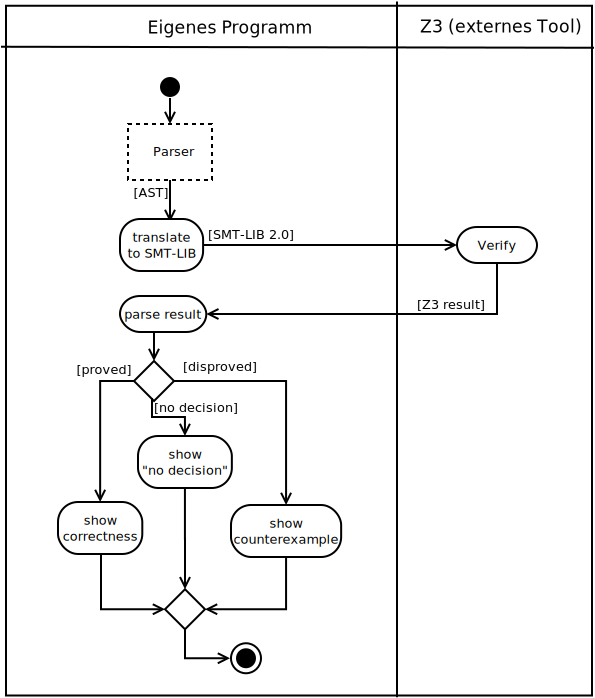
\includegraphics[scale=0.5]{images/AktivitaetSMTTranslator.pdf}\\\\
Zur "uberpr"ufung der Korrektheit des Programms wird Z3 benutzt. 
\begin{enumerate}
\item Zuerst wird das Programm geparst (siehe Aktivit"atsdiagramm Parser/Type-Checker).
\item Im Fehlerfall ist keine "Uberpr"ufung durch Z3 m"oglich. Im Erfolgsfall wird der durch den Parser generierte AST an den SMTLib-Translator gegeben.
\item Der SMTLib-Translator "ubersetzt das Programm inklusive Spezifikation ins SMTLib-2.0-Format. Dieses bildet die Eingabe f"ur Z3.
\item Die von Z3 zur"uckgegebene Antwort wird vom Result-Parser analysiert.
\item Meldet der Beweiser die Korrektheit des Programms oder konnte er keine Entscheidung treffen, wird dieses Ergebnis dem Benutzer bekannt gegeben. Falls der Beweiser das Programm falsifizieren konnte, wird dem Benutzer das Ergebnis zusammen mit einem m"oglichen Gegenbeispiel angezeigt.
\end{enumerate}

\section{Zustandsdiagramm}

Das folgende Zustandsdiagramm zeigt das Verhalten des Systems bei Benutzeraktionen. \\
\includegraphics[scale=0.9]{images/Zustand.pdf}
\begin{itemize}
\item Beim Starten des Programms geht dieses in den "`idle"'-Zustand. Hier l"auft der Interpreter nicht, und es ist kein Programmzustand gespeichert. Falls einer vorhanden ist, wird dieser beim Eintritt in den "`idle"'-Zustand gel"oscht.
\item Beim Ausw"ahlen von "`single step"' wird das Userprogramm geparst und ein Statement wird ausgef"uhrt, nachdem der Zustand "`single step"' betreten worden ist. Ist kein Statement mehr vorhanden, so beendet sich der Interpreter, das Programm geht zur"uck in den Zustand "`idle"'. Sonst wird nach Ausf"uhren des Statements das Programm pausiert, der Zustand "`paused"' wird eingenommen.
\item Beim Eintritt in den "`paused"'-Zustand wird der Zustand des Userprogramms ausgegeben. W"ahrend der Pausierung l"auft der Interpreter nicht. In diesem Zustand stehen die gleichen M"oglichkeiten wie im "`idle"'-Zustand zu Verf"ugung, das Parsen bei Verlassen des Zustands entf"allt aber.
\item Wenn im "`idle"'-Zustand "`run to breakpoint"' aufgerufen wird, wird das Userprogramm geparst und das Programm geht in den Zustand "`run"'. Das Userprogramm wird solange ausgef"uhrt, bis es zu Ende ist (neuer Zustand: "`idle"') oder der Interpreter pausiert, ein Breakpoint getroffen oder eine Assertion falsifiziert wird. In diesen F"allen ist der neue Zustand "`paused"'.
\item In jedem Zustand au"ser "`idle"' ist es zus"atzlich m"oglich, das Userprogramm abzubrechen, wobei der Interpreter beendet wird und alle vorhandenen Variablen-Informationen gel"oscht werden. Das Programm geht danach in den Zustand "`idle"'.
\item In jedem Zustand kann das Programm durck einen Klick auf den Exit-Button beendet werden.
\end{itemize}
\newpage

\section{Sequenzdiagramme}
\subsection{Besucher-Muster}
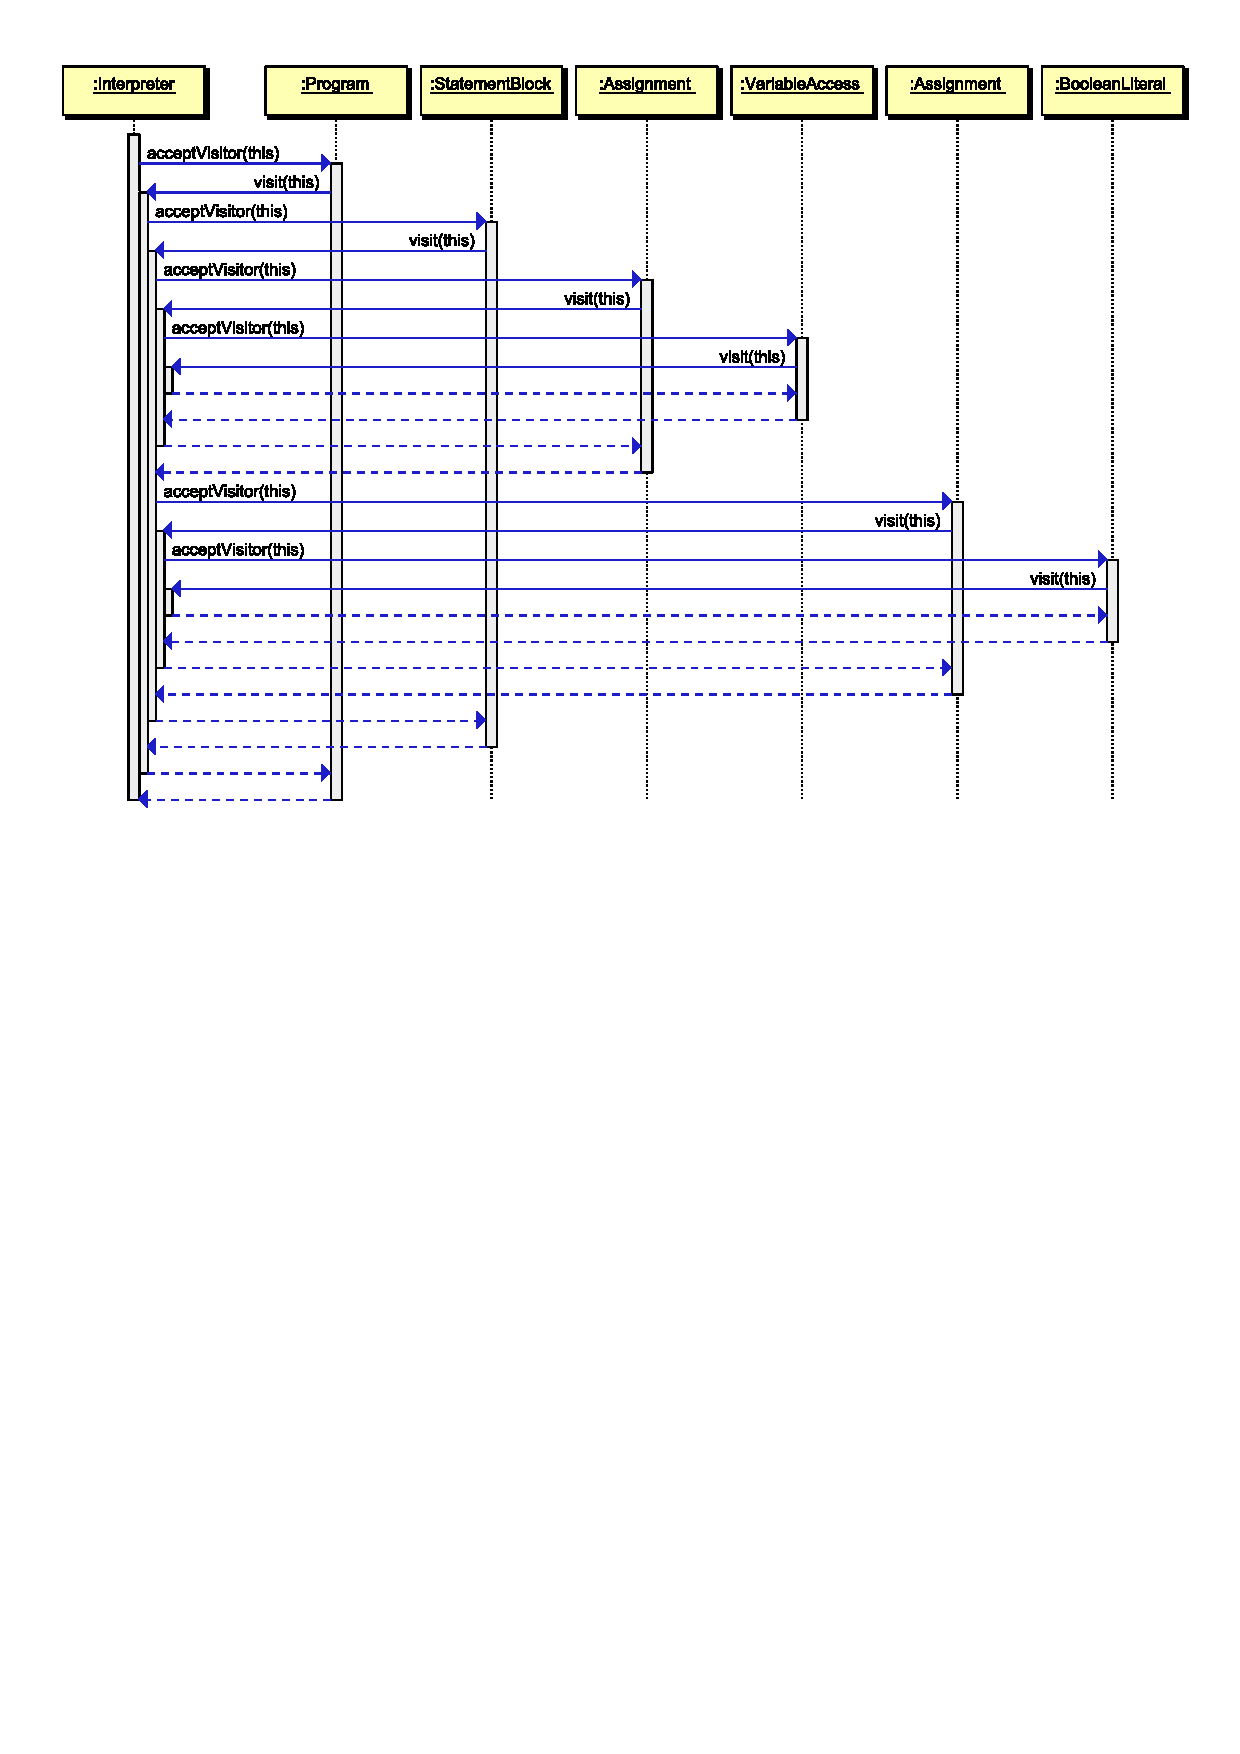
\includegraphics[scale=0.9]{images/visitor_pattern.pdf} \newline
Dieses Sequenzdiagramm zeigt die Arbeitsweise des Besuchermusters an einem Beispiel. Dies ist zum Beispiel das Statement "`flag = true | false"'.
\begin{itemize}
\item Der Interpreter wird mit dem momentanen Programmzustand aufgerufen und ruft den Getter f"ur das aktuelle Statement auf.
\item Der Besucher ruft die accept-Methode darauf auf, welche ihrerseits die richtige visit-Methode aufruft.
\item Bei visit(Assignment) wird zuerst der hintere Ausdruck ausgewertet (hier: "`true | false"').
\item F"ur diese Expression wird eine neue visit-Methode aufgerufen. Diese besucht zuerst die erste Subexpression, "uberpr"uft den Operanden, ob er un"ar oder bin"ar ist. Da er binär ist, wird auch die zweite Subexpression besucht.
\item Nachdem der Ausdruck ausgewertet worden ist, wird der letzte Bearbeitungsschritt der Zuweisung durchgef"uhrt. Dazu wird der Variablenname gebraucht (assignment.getVar().getName()). Dann wird die Variable im State neu gesetzt.
\item Der neue Zustand wird zur"uckgegeben.
\end{itemize}

\subsection{Breakpoints}
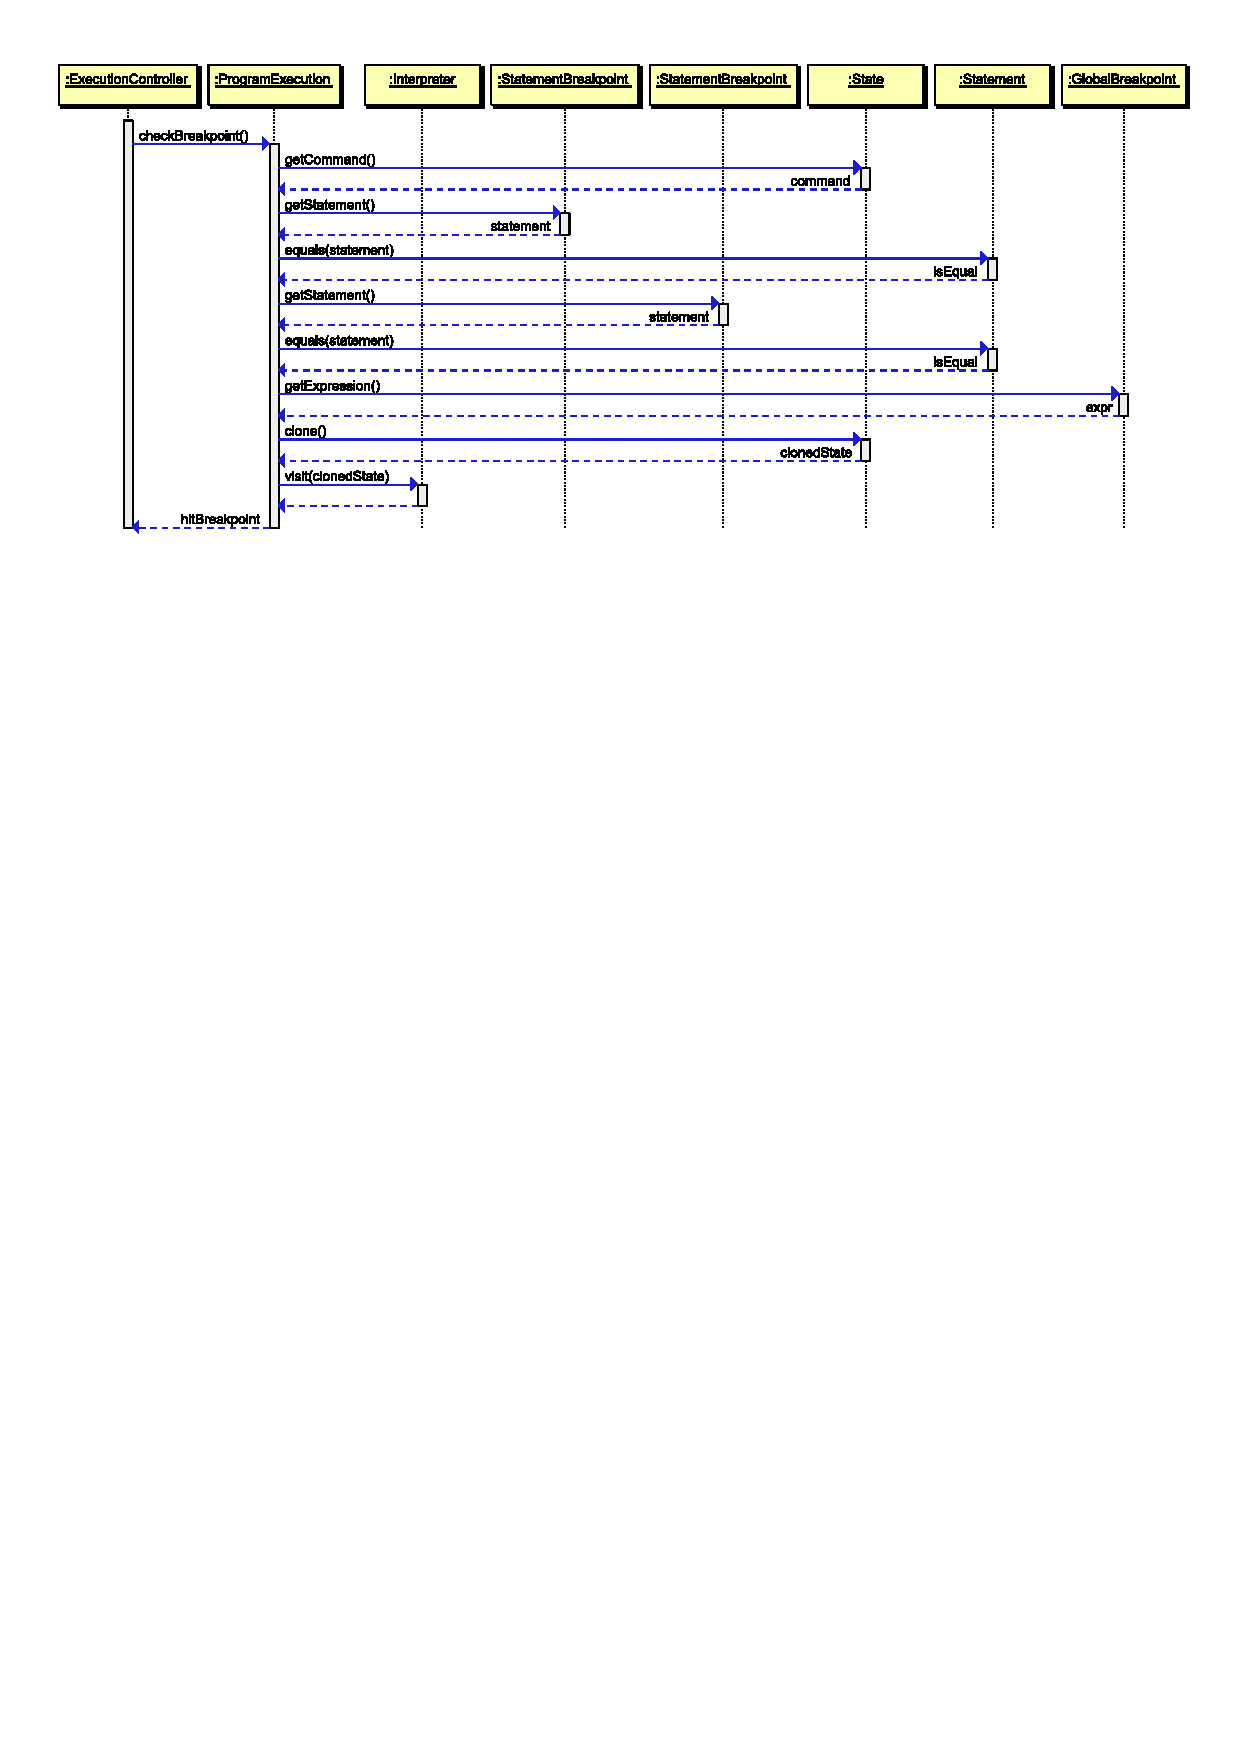
\includegraphics[scale=0.9]{images/Breakpoints.pdf} \newline
\begin{itemize}
\item Dieses Sequenzdiagramm zeigt, wie die Breakpoints ausgewertet werden. Daf"ur wird angenommen, dass zwei Statement-Breakpoints und ein globaler Breakpoint aktiv sind.
\item Zuerst ruft die Instanz von ProgramExecution die Methode getCommand von State auf, um das aktuelle Statement zu bekommen.
\item F"ur jeden einem Statement zugeordneten Breakpoint wird dieses Statement abgefragt und mit dem aktuell auszuf"uhrenden verglichen.
\item Danach wird f"ur jeden globalen Breakpoint die ihm zugeordnete Bedingung angefordert. State wird geklont, und die Bedingung wird mit der geklonten State-Instanz vom Interpreter ausgewertet.
\item Der R"uckgabewert von checkBreakpoint() ist genau dann ja, falls mindestens ein Breakpoint getroffen wurde.
\end{itemize}

\subsection{Interpreter-Initialisierung}
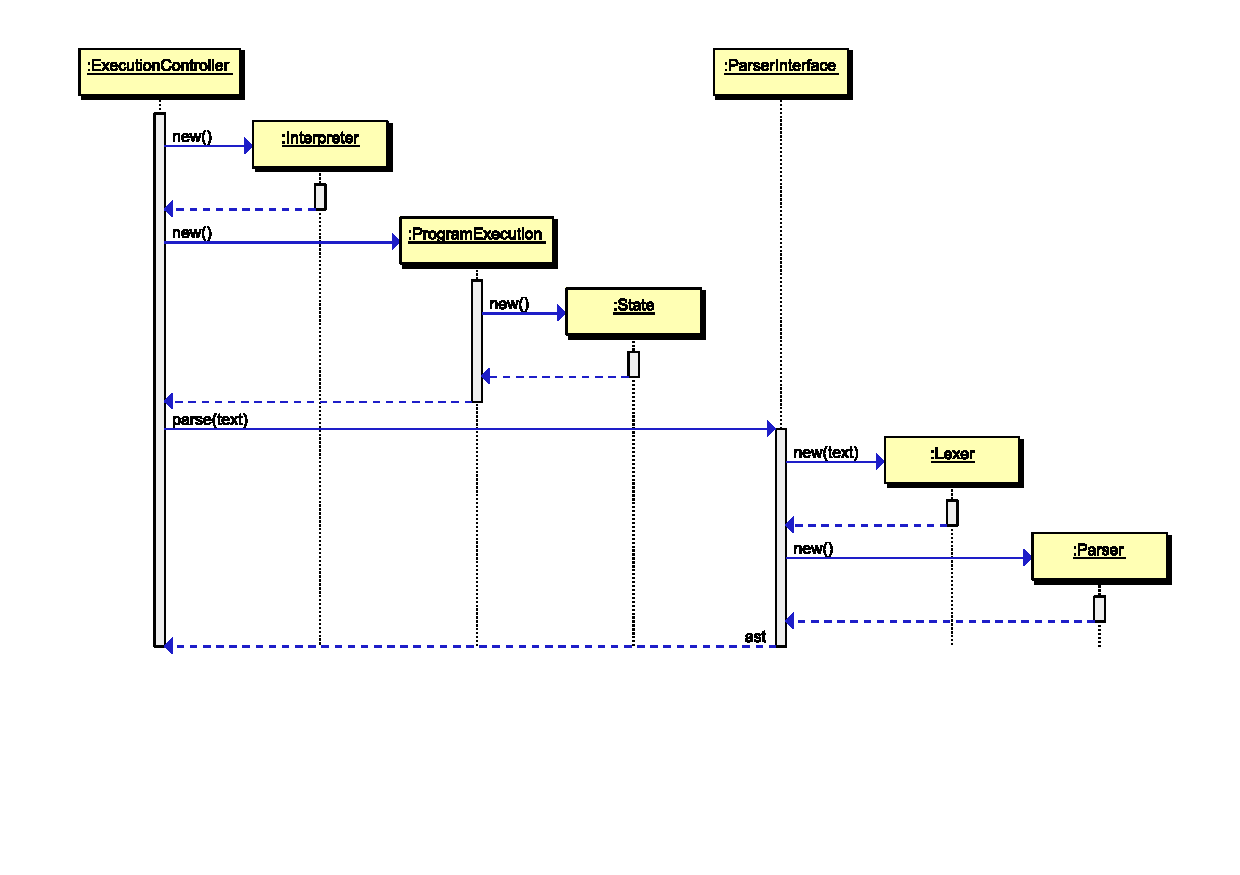
\includegraphics[scale=0.9]{images/interpreter_init.pdf} \newline
\begin{itemize}
\item Dieses Sequenzdiagramm zeigt die Initialisierung des Interpreters bei Programmstart.
\item Der ExecutionController erzeugt jeweils eine neue Instanz von Interpreter und ProgramExecution, wobei letztere eine neue State-Instanz erzeugt.
\item Dann wird das Parserinterface aufgerufen, welches eine Instanz des Lexers f"ur diesen Parse-Vorgang erzeugt. Der Parser erzeugt daraus einen AST.
\item Dieser wird vom TypeChecker auf Typkorrektheit "uberpr"uft.
\end{itemize}

\subsection{Start-Button}
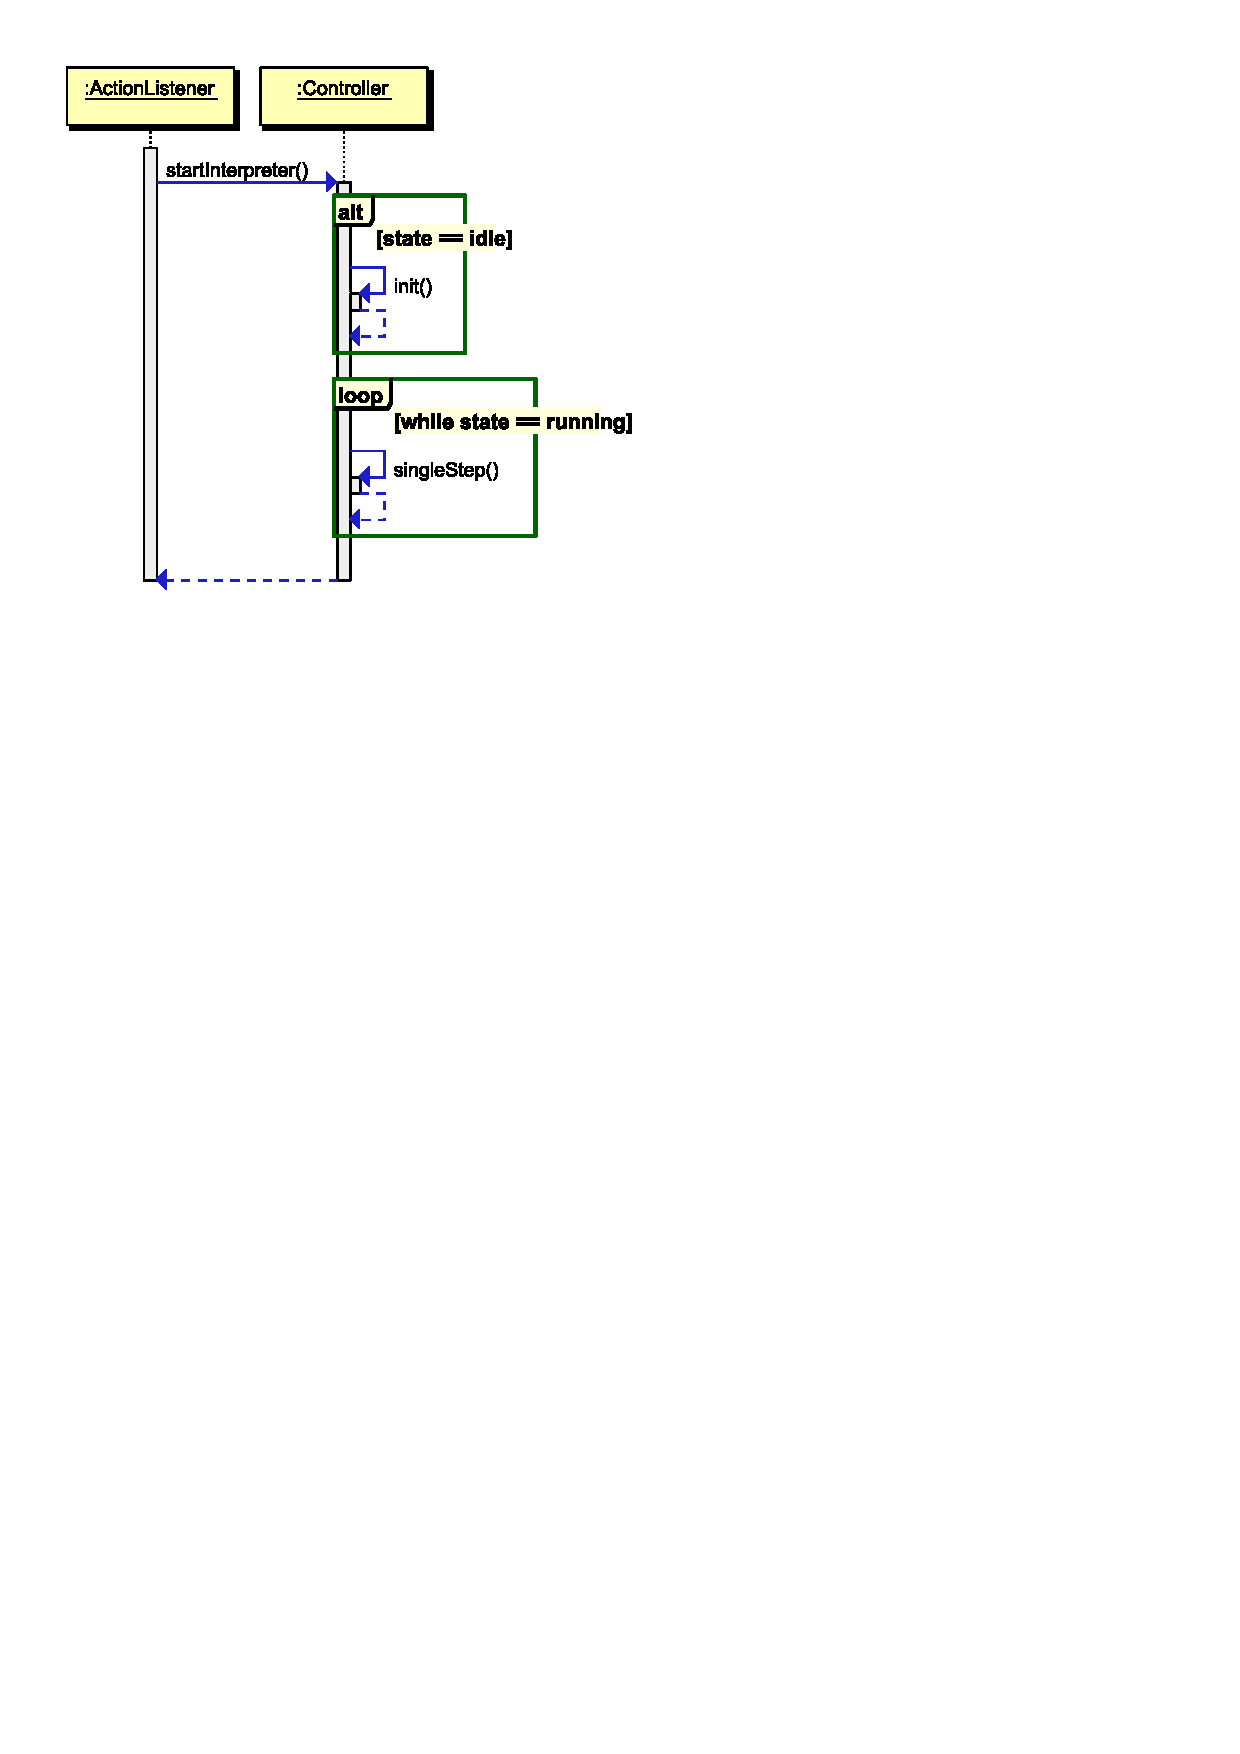
\includegraphics[scale=0.9]{images/Button_play.pdf} \newline
\begin{itemize}
\item Beim Dr"ucken auf den Play-Button wird der entsprechende ActionListener ausgef"uhrt, welcher die startInterpreter-Methode des ExecutionController ausf"uhrt.
\item Ist das Programm noch nicht geparst worden, wird der Interpreter initialisiert (s. letztes Diagramm).
\item Danach wird das Programm schrittweise (s. n"achstes Diagramm) ausgef"uhrt, wobei vor jedem Einzelschritt gepr"uft wird, ob ein Breakpoint getroffen oder das Programm pausiert wurde. Letzteres wird "uber das Beobachter-Muster realisiert.
\end{itemize}

\subsection{Single-Step-Button}
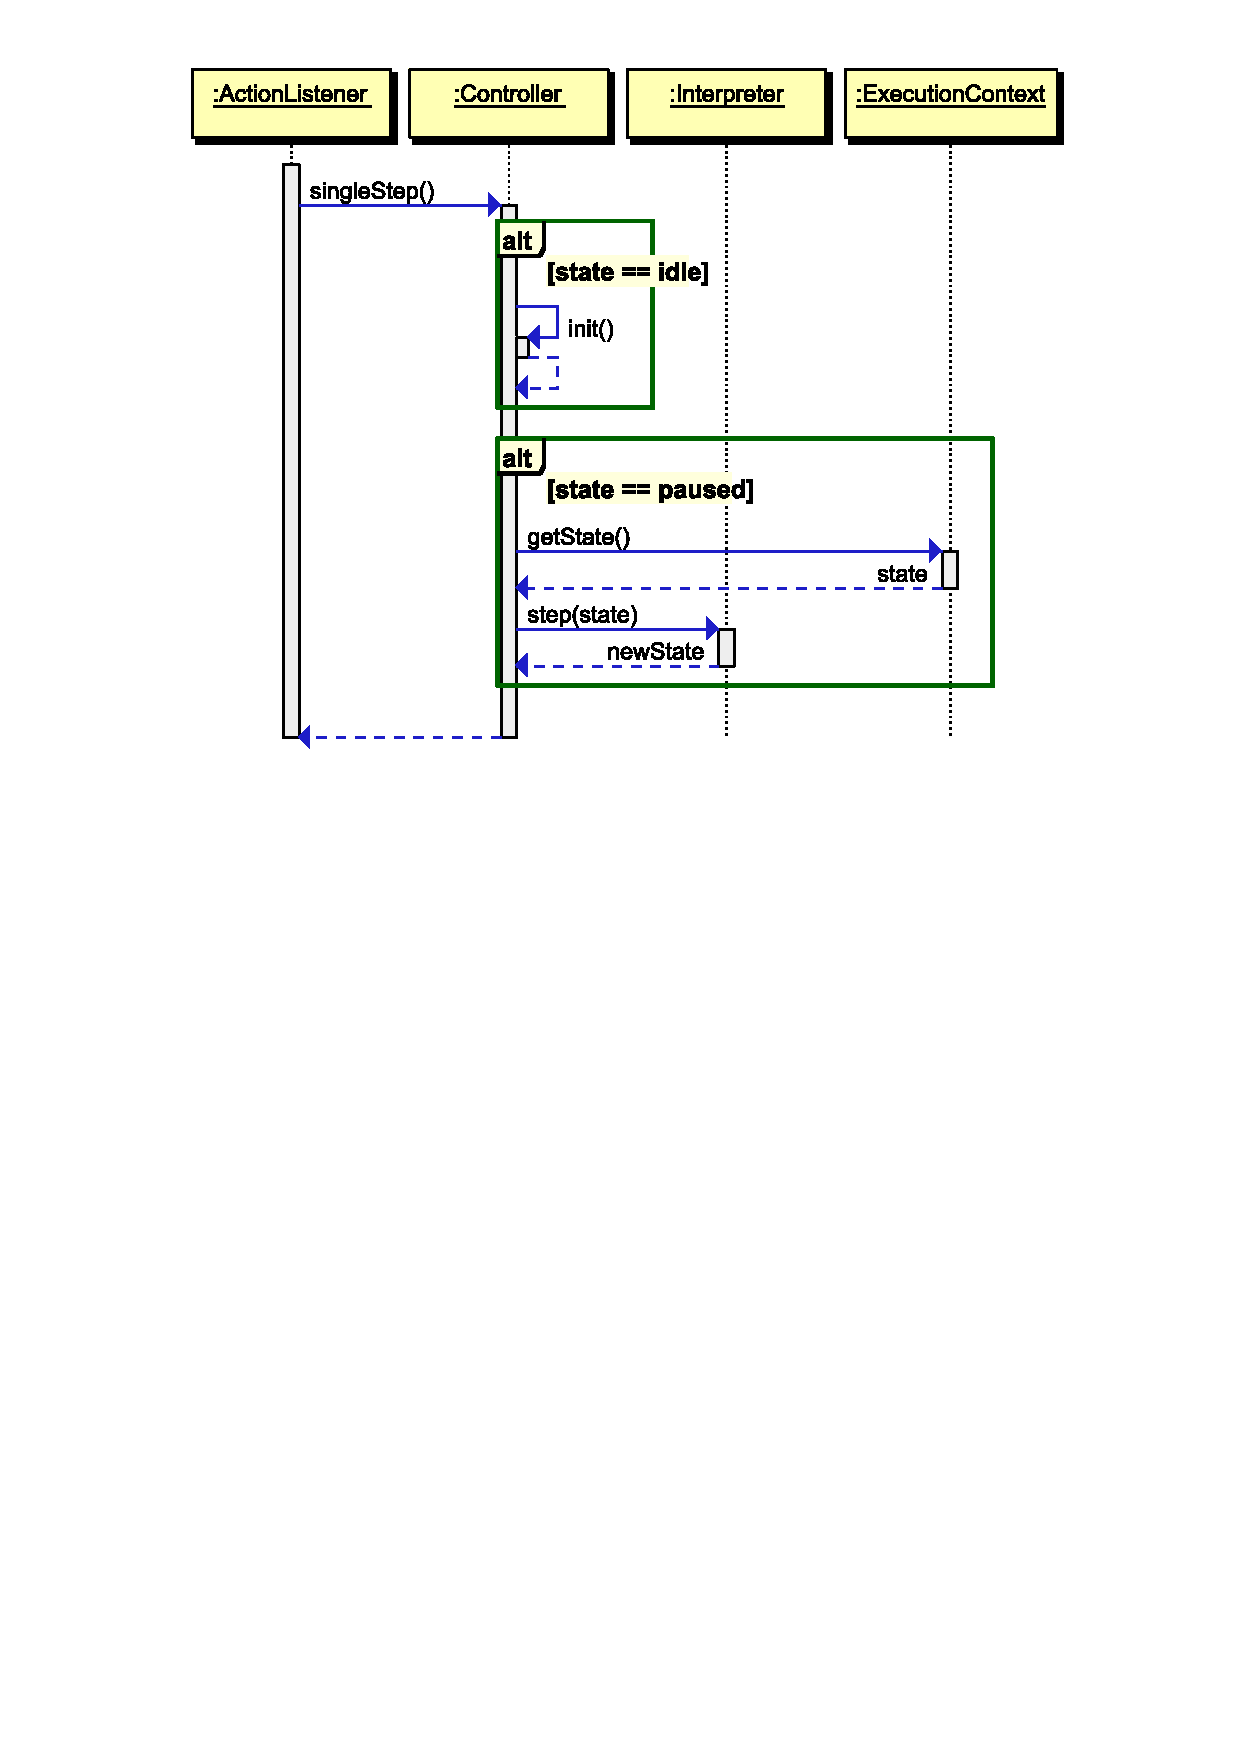
\includegraphics[scale=0.9]{images/Button_singleStep.pdf} \newline
\begin{itemize}
\item Beim Dr"ucken auf den SingleStep-Button wird der entsprechende ActionListener ausgef"uhrt, welcher die singleStep-Methode des ExecutionController ausf"uhrt.
\item Ist das Programm noch nicht geparst worden, wird der Interpreter initialisiert (s. entsprechendes Diagramm).
\item Danach wird ein Einzelschritt des Programms ausgef"uhrt. Daf"ur wird der im ProgramExecution gekapselte Progammzustand abgefragt und an den Interpreter gegeben; der neue Zustand wird dann wieder zur"uckgespeichert.
\end{itemize}

\newpage
\section{Erweiterbarkeit}
Die Schnittstelle zum Beweiser ist so ausgelegt, dass jeder Beweiser, der das SMT LIB 2.0 Format unterst\"{u}tzt, verwendet werden kann und f\"{u}r eine weitere Anbindungen nur wenige \"{A}nderungen n\"{o}tig sind.
Durch die gering gehaltenen Schnittstell des Parsers kann dieses Paket leicht ge\"{a}ndert oder ersetzt werden, ohne dass der Rest des Programms davon beeinflusst wird.
Die While-Sprache ist durch ihre Grammatik festgelegt. Eine Erweiterung dieser Grammatik ist kein Problem f\"{u}r das Programm. Man kann die Sprache modifizieren und neue Befehle definieren. Dies wird weiter durch den Einsatz des Visitor-Patterns f�r Interpreter, Typchecker und Beweiseranbindung beg�nstigt, da hierdurch f�r jedes weitere Syntaxelement der Sprache nur eine Methode pro Programmelement, dass den abstrakten Syntaxbaum traversiert, implementiert werden muss. Auch das Hinzuf\"{u}gen und \"{A}ndern von Typen f\"{u}r diese Sprache ist problemlos m\"{o}glich.

\section{Struktur der While-Sprache}
\includegraphics[scale=1]{images/DependencyGraph.pdf}

\section{Syntax der While-Sprache}
\VerbatimInput{WhileLanguage.g}

\begin{landscape}
\section{Implementierungsplan}
\subsection{Vorgangsliste}
\includegraphics[scale=0.7]{images/Implementierung_Vorgangsliste_1.pdf}
\newpage
\includegraphics[scale=0.7]{images/Implementierung_Vorgangsliste_2.pdf}
\newpage
\subsection{Gantt-Diagramm}
\includegraphics[scale=0.7]{images/Implementierung_Gantt.pdf}
\end{landscape}

\end{document}
